
% \documentclass[review=false, screen=true]{acmart}
\documentclass[format=acmsmall, review=false, screen=true]{acmart}

% Set letter paper size:
% \setlength{\paperheight}{11in}
% \setlength{\paperwidth}{8.5in}
% \usepackage[
%   % pass,% keep layout unchanged 
%   % showframe,% show the layout
%   % a4paper
% ]{geometry}


% Package to generate and customize Algorithm as per ACM style
\usepackage[linesnumbered,ruled,vlined]{algorithm2e}
% \usepackage[ruled]{algorithm2e}
\renewcommand{\algorithmcfname}{ALGORITHM}
\SetAlFnt{\small}
\SetAlCapFnt{\small}
\SetAlCapNameFnt{\small}
\SetAlCapHSkip{0pt}
\IncMargin{-\parindent}



\usepackage{booktabs}
\usepackage{tabularx}  

\usepackage{amsmath,amssymb,amsfonts}

\usepackage{enumitem}

\usepackage{lipsum} 

\SetKwRepeat{Do}{do}{while} 


\usepackage{lmodern}
\usepackage{courier}

\usepackage{listings}
\lstset{
  language={Pascal},
  backgroundcolor=\color{white},   % choose the background color; you must add \usepackage{color} or \usepackage{xcolor}; should come as last argument
  basicstyle=\ttfamily\small,      %\footnotesize,        % the size of the fonts that are used for the code
  breakatwhitespace=false,         % sets if automatic breaks should only happen at whitespace
  breaklines=true,                 % sets automatic line breaking
  captionpos=b,                    % sets the caption-position to bottom
  commentstyle=\color{red},        % comment style
  frame=single,                    % adds a frame around the code
  keepspaces=true,                 % keeps spaces in text, useful for keeping indentation of code (possibly needs columns=flexible)
  keywordstyle=\color{blue},       % keyword style
  language=Octave,                 % the language of the code
  showspaces=false,                % show spaces everywhere adding particular underscores; it overrides 'showstringspaces'
  showstringspaces=false,          % underline spaces within strings only
  showtabs=false,                  % show tabs within strings adding particular underscores
  stringstyle=\color{brown},       % string literal style
  tabsize=2,                       % sets default tabsize to 2 spaces
}

\usepackage{setspace}



% % Metadata Information
\acmJournal{CSUR}
\acmVolume{0}
\acmNumber{0}
\acmArticle{1}
\acmYear{2020}
\acmMonth{12} 
% \copyrightyear{2009}


% % Copyright
% \setcopyright{acmcopyright}
% \setcopyright{acmlicensed}
% %\setcopyright{rightsretained}
% %\setcopyright{usgov}
% %\setcopyright{usgovmixed}
% %\setcopyright{cagov}
% %\setcopyright{cagovmixed}
\setcopyright{none}

% % DOI
% \acmDOI{0000001.0000001} 

% % Paper history
% \received{February 2007}
% \received[revised]{March 2009}
% \received[accepted]{June 2009}


% Document starts
\begin{document} 
% Title portion. Note the short title for running heads 
\title[Title]{COSC 4P14 -- Assignment 4 -- StudentID}  
% \title[Energy-Efficient Offloading in Mobile Cloud Computing System]{Energy-efficient Offloading in Mobile Cloud Computing System}  

\author{Author Name}
\affiliation{%
  \institution{Brock University}
  \streetaddress{1812 Sir Isaac Brock Way}
  \city{St. Catharines}
  \state{ON}
  \postcode{L2S 3A1}
  \country{Canada}
}

\begin{abstract}

Abstract text...

\end{abstract}




%  \begin{CCSXML}
%   <ccs2012>
%     <concept>
%       <concept_id>10003033.10003099.10003100</concept_id>
%       <concept_desc>Networks~Cloud computing</concept_desc>
%       <concept_significance>500</concept_significance>
%     </concept>
%     <concept>
%       <concept_id>10003033.10003106.10003113</concept_id>
%       <concept_desc>Networks~Mobile networks</concept_desc>
%       <concept_significance>300</concept_significance>
%     </concept>
%     <concept>
%       <concept_id>10010520.10010521.10010537.10003100</concept_id>
%       <concept_desc>Computer systems organization~Cloud computing</concept_desc>
%       <concept_significance>500</concept_significance>
%     </concept>
%     <concept>
%       <concept_id>10011007.10010940.10010941.10010949.10010957.10010688</concept_id>
%       <concept_desc>Software and its engineering~Scheduling</concept_desc>
%       <concept_significance>500</concept_significance>
%     </concept>
%     <concept>
%       <concept_id>10011007.10010940.10010971.10011120.10003100</concept_id>
%       <concept_desc>Software and its engineering~Cloud computing</concept_desc>
%       <concept_significance>300</concept_significance>
%     </concept>
%     <concept>
%       <concept_id>10002951.10003152.10003517.10003176</concept_id>
%       <concept_desc>Information systems~Cloud based storage</concept_desc>
%       <concept_significance>100</concept_significance>
%     </concept>
%     <concept>
%       <concept_id>10002951.10003227.10003245</concept_id>
%       <concept_desc>Information systems~Mobile information processing systems</concept_desc>
%       <concept_significance>100</concept_significance>
%     </concept>
%   </ccs2012>
% \end{CCSXML}

% \ccsdesc[500]{Networks~Cloud computing}
% \ccsdesc[300]{Networks~Mobile networks}
% \ccsdesc[500]{Computer systems organization~Cloud computing}
% \ccsdesc[500]{Software and its engineering~Scheduling}
% \ccsdesc[300]{Software and its engineering~Cloud computing}
% \ccsdesc[100]{Information systems~Cloud based storage}
% \ccsdesc[100]{Information systems~Mobile information processing systems}

%
% End generated code
%

% \texorpdfstring

% \keywords{Vehicular Cloud Computing, Resource Management, Resource Scheduling.}



\maketitle


\section{Network Security Questions}

Add your assignment answers here... Include tables, algorithms, and figures if needed...

\begin{figure}[h!]
  \centering
  \includegraphics[width=0.3\linewidth]{images/rosette.eps} 
  \caption{Example of an image. (you can construct more sophisticated layouts using subfigs)}
\end{figure}

\begin{table}[h]
  \centering
  % \small
  \caption{Example of a table (nicely looking tables with booktabs).}
  \begin{tabular}{llll} %p{1.7cm}
    \toprule
    \textbf{Name} & \textbf{ID} & \textbf{Subtotal} & \textbf{Total} \\  
    \midrule
  John Doe & jd2001 & 75  & 89 \\
    \bottomrule
  \end{tabular}
\end{table}  

\begin{algorithm}[t]
  \footnotesize
  \caption{Example of algorithm}
  \label{algo1}
  \KwData{$X_i$; $P_{a_i}$; $R$; $A_i$; $\gamma$; $\epsilon$ }
  \KwResult{$\pi_i$; $v^*$ } 

  $V=0$; $\pi_i=0$\;
  \Do{$\Delta < \epsilon$}{
    $\Delta = 0$\;
    \For{$x \in X$}{
      $Av=0$\;
      \For{$a \in A$}{
        $x_{n} = A(x)$\;
        $Av[a] = P_a[x][x_{n}]*(R[x_{n}]+\gamma*V[x_{n}])$\;
      }
      $av_{best} = max(Av)$\;
      $\Delta = max(\Delta, |av_{best}-V[x]|)$\;
      $V[x] = av_{best}$\;
      $\pi_i[x]=argmax(Av)$\;
    }
  }
\end{algorithm}


\subsection{Question 1}

\lipsum[2-4]



\section{Secured Java Application}

The description of your Java code is here... Include any auxiliary text object for aiding your description (tables, algorithms, figures...)

Do not forget to cite sources~\cite{GnutellaNet2002} if any!


\subsection{Performance Analysis}

\lipsum[2-4]


\subsection{Conclusions}


\bibliographystyle{ACM-Reference-Format-Journals}
\bibliography{acmsmall-sample-bibfile}


\appendix

\section{HelloWorld - Use lstlisting environment to add your Java code}
\begin{spacing}{0.8}
\begin{lstlisting}[language=Java]
public class HelloWorld {
    public static void main(String[] args) {
        // Prints "Hello, World" to the terminal window.
        System.out.println("Hello, World");
    }
}
\end{lstlisting}
\end{spacing} 

\clearpage

\section{Class2}

\end{document}
